\section{Results}

\subsection{Visualisation}

We were able to develop command-line programs to show both the kernelization
and branching algorithms working in real-time. The speed of the algorithms has
been slowed to allow the user to see and understand what is happening at each
step. Both programs take a path to an edge list file and a \(k\) value as
command-line arguments, so visualisations can be produced of different graphs
at various \(k\) values. This gives us the ability to see how a kernel of a
graph changes depending on the value of \(k\).

Naturally, there is a limit to the size of the graph being displayed. This is
because on top of the memory required to store the entire graph and to run each
algorithm, memory is also needed for rendering the image for each frame.

\subsubsection{Kernelization}

Being the visually more exciting and intricate algorithm, it made sense for us
to focus our efforts on the kernelization algorithm. In Figure
\ref{fig:kernelization_visualisation}, you can see that we have split the plot
into two. On the left side, we show the entire graph, marking which vertices
and edges have been added to the kernel as well as which edge of the graph is
currently being processed. A subtitle shows the number of nodes and edges in
the graph. On the right, we show the kernel being built up as the algorithm
progresses. All vertices and edges of the kernel exist in the same position as
they do in the graph, so it is easy to see how it resembles the core components
of the whole graph once enough vertices have been added. Red marks those
vertices and edges that are part of the maximal matching that the kernelization
algorithm maintains. Black marks the neighbours of each matched vertex. The
subtitle also shows information relating to the kernel at each step as well as
how the kernel relates to the graph in terms of its size.

\begin{figure}[htb]
    \centering
    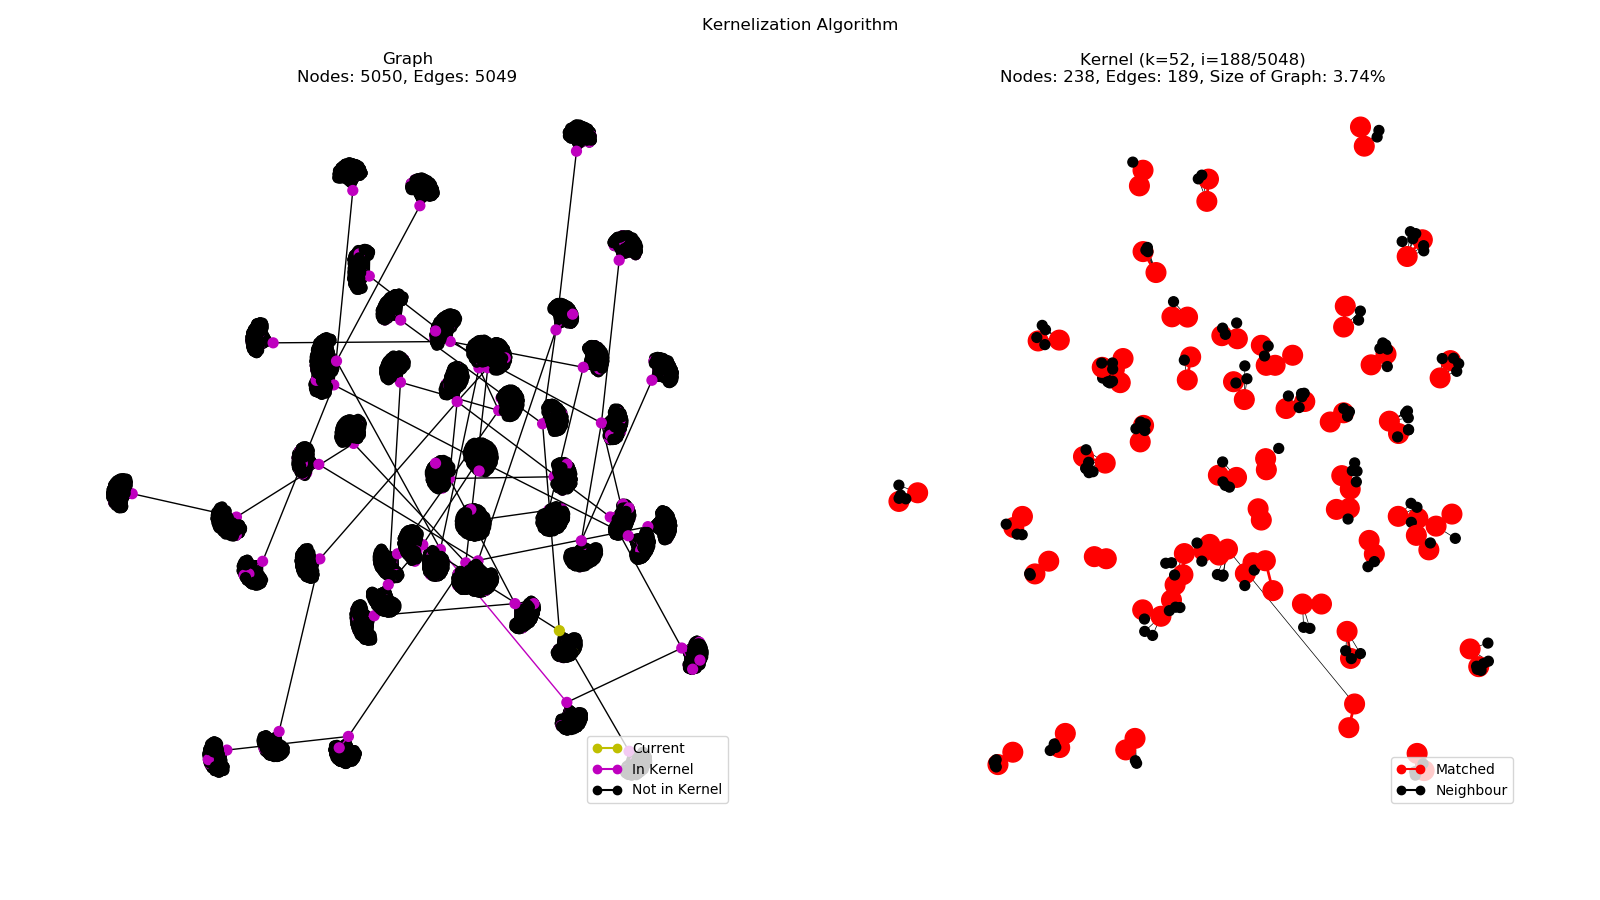
\includegraphics[width=\textwidth]{visuals_kernelization.png}
    \caption{Streaming Kernelization Visualisation}
    \label{fig:kernelization_visualisation}
\end{figure}

Some considerations were made in choosing how the graphs were drawn. Graph
drawing, being its own area of study, we did not have much control other than
choosing which algorithm looked better. Kamada-Kawai \cite{kamada1989drawing}
worked well for smaller graphs (roughly $< 1000$) but required too much memory
for bigger ones, so we had to resort to using Spring (also known as the
Fruchterman-Reingold force-directed algorithm) \cite{fruchterman1991graph}.

While the method we chose for creating live demonstrations was rather crude,
Matplotlib does include classes for creating animations with that can then be
exported into video formats. Using this, we ported over the code used to
generate the live demonstration into a new program that creates videos exported
to whichever format is specified. This allows for easy sharing of GIFs showing
the kernelization in practice.

\subsubsection{Branching}

The branching algorithm is much simpler visually. We created a live
demonstration that shows the search tree and the depth-first search being
applied to it. The yellow vertex marks the current vertex cover configuration
being tested and a boldened trail of edges shows the current path being taken.
The binary string being used for the path is shown towards the top left with an
underscore under the current binary value, below that is the current edge of
the stream. A subtitle shows the current depth and edge index.

\begin{figure}[htb]
    \centering
    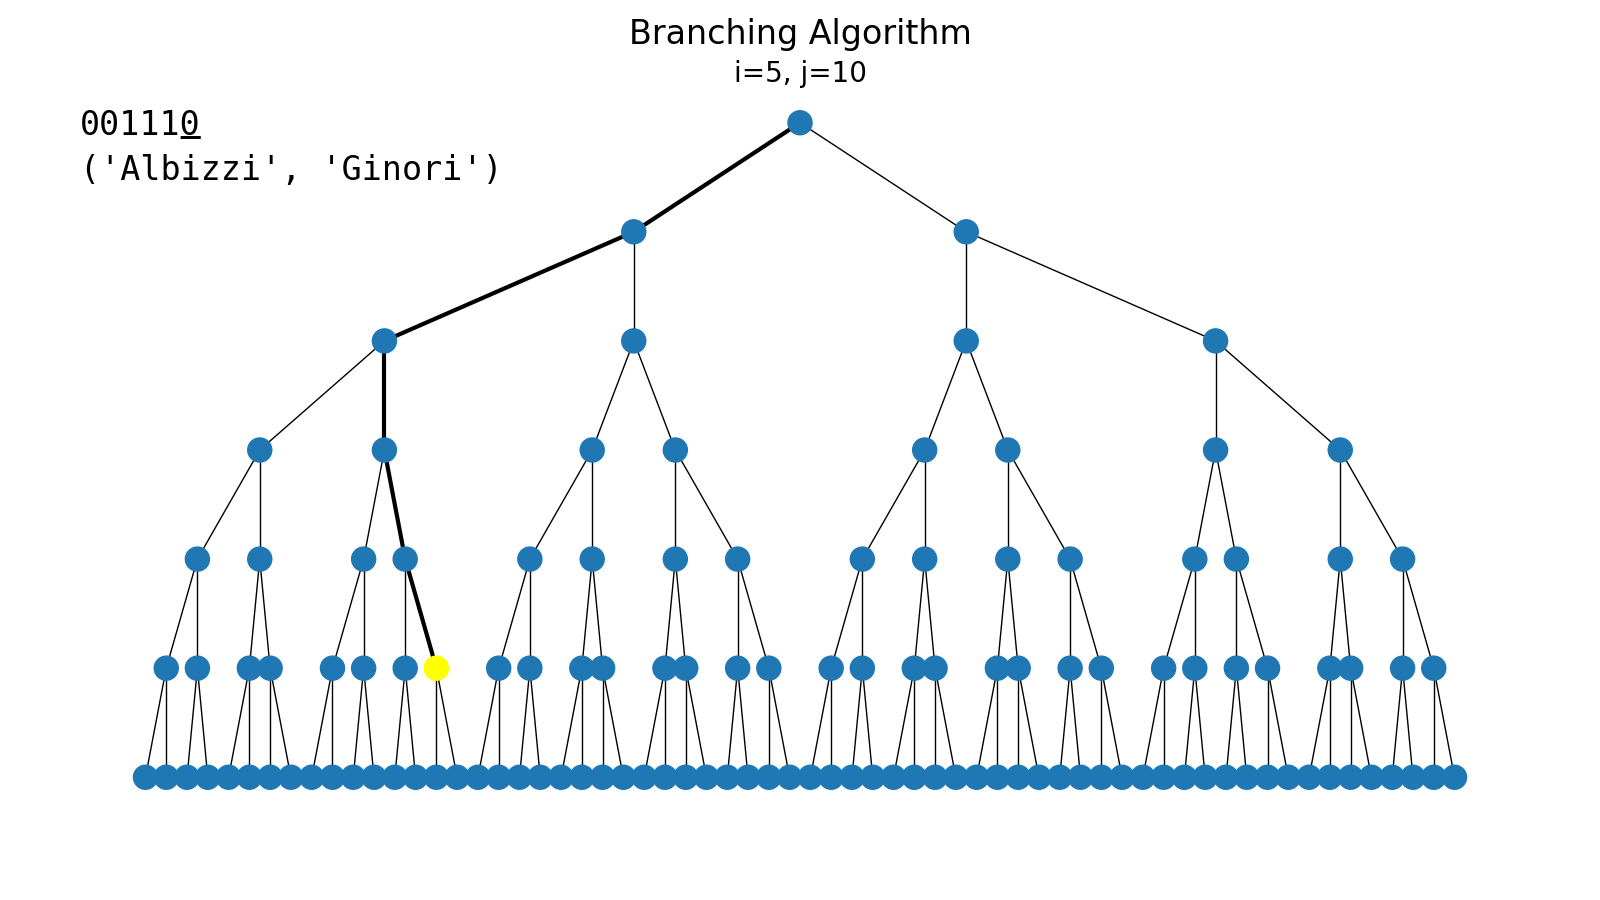
\includegraphics[width=\textwidth]{visuals_branching.png}
    \caption{Streaming Branching Visualisation}
    \label{fig:branching_visualisation}
\end{figure}

To draw the tree, we used Graphviz \cite{ellson2003graphviz}, a graph
visualisation program that has many built-in layouts. We used the "dot" layout
for the hierarchical layout of a tree.

It should be noted that, due to the exponential nature of trees, a \(k\) value
of 10 or more will take significantly longer to load. As such, it is advised to
use only the visualisation for \(k\) values smaller than this. From Figure
\ref{fig:branching_visualisation} you can see that at \(k=6\), the bottom line
of vertices is already getting cramped for space.

\subsection{Performance Benchmarking}

\subsubsection{Memory Profiling}

We were able to get quite telling memory profiles of both of the algorithms.
For each, the stream algorithms are labelled by light blue square brackets in
the plot for when the function starts and ends. Similarly, the classical
algorithms are labelled in light green. Time is plotted along the x-axis and
memory usage along the y-axis. The red lines mark when peak memory usage occurs.

\begin{figure}[htb]
    \centering
    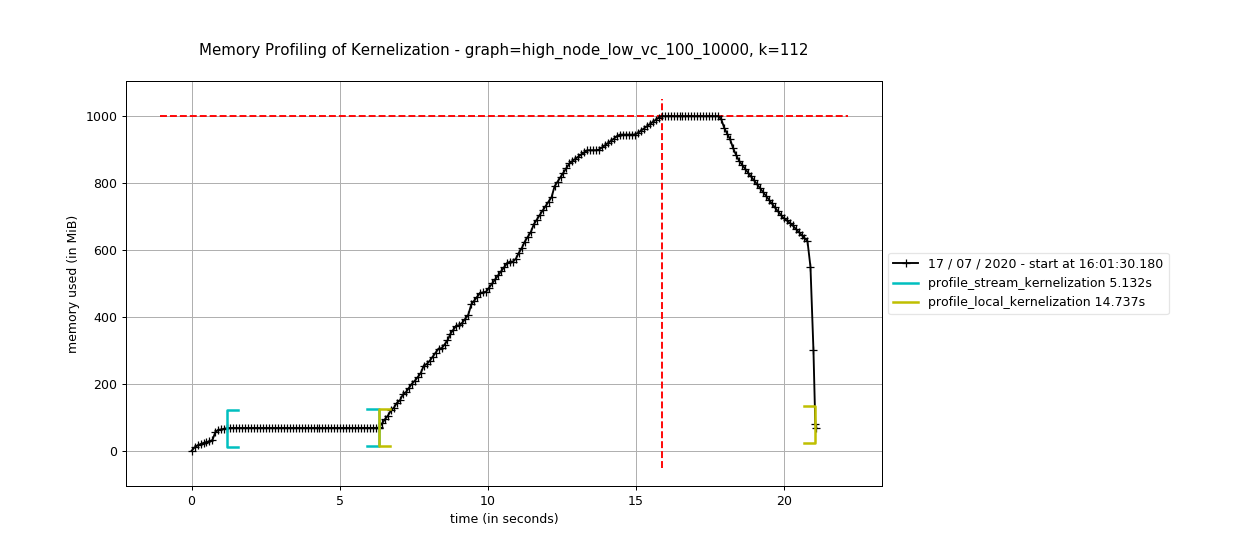
\includegraphics[width=\textwidth]{benchmark_memory_kernelization_100_10000.png}
    \caption{Memory Profiling of Kernelization}
    \label{fig:benchmark_mem_kernelization}
\end{figure}

Figure \ref{fig:benchmark_mem_kernelization} shows the kernelization algorithm.
As you can see the stream function has seemingly fixed memory usage throughout
its processing while the classical function climbs rapidly.

\begin{figure}[htb]
    \centering
    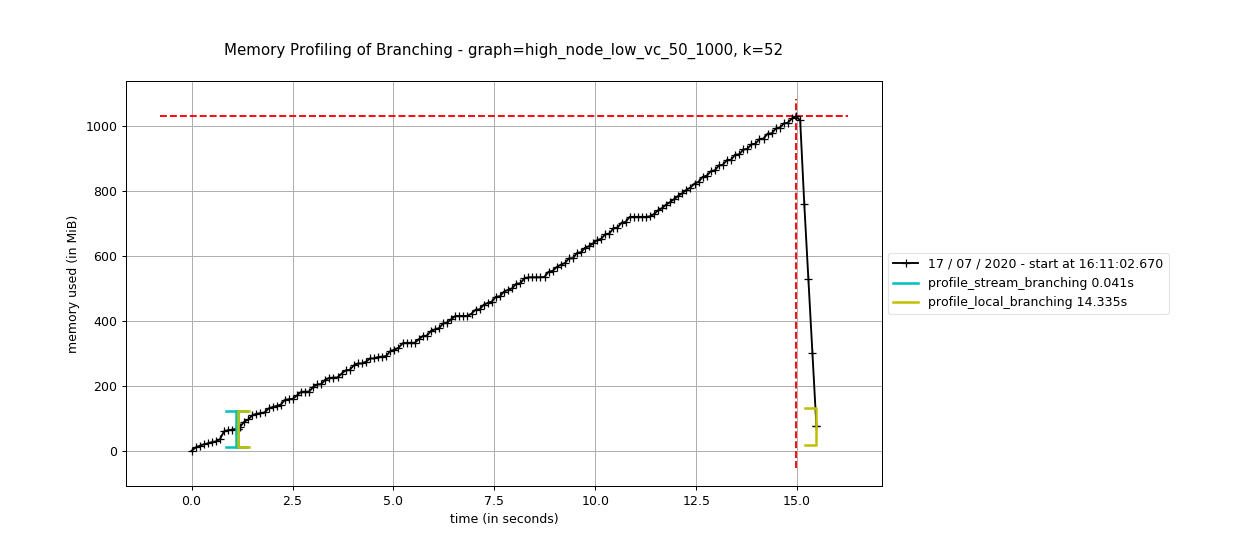
\includegraphics[width=\textwidth]{benchmark_memory_branching_50_1000.png}
    \caption{Memory Profiling of Branching}
    \label{fig:benchmark_mem_branching}
\end{figure}

Figure \ref{fig:benchmark_mem_branching} shows the branching algorithm. The
stream function finished almost instantaneously with no discernible change in
memory usage while the classical function continued to climb through it's
processing.

\subsubsection{Runtime Analysis}

Results for runtime analysis are rather more even than memory usage, which is
expected. Though, the stream functions do still pull ahead fairly consistently
at all graph sizes. We were able to test all algorithms with a wide range of
graph sizes as well as \(k\) values to get a better picture of how they perform
under different circumstances.

\begin{figure}[htb]
    \centering
    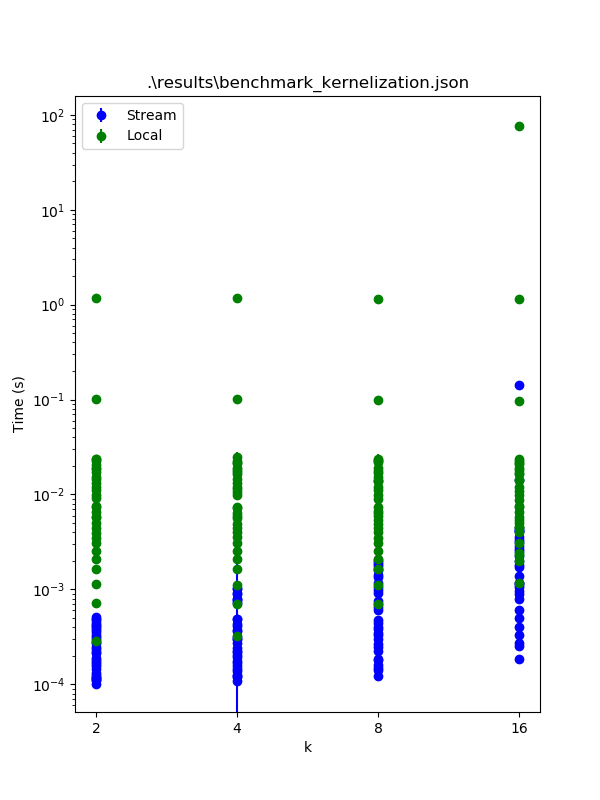
\includegraphics[width=\textwidth]{benchmark_time_kernelization.png}
    \caption{Runtimes of Kernelization}
    \label{fig:benchmark_time_kernelization}
\end{figure}

Figure \ref{fig:benchmark_time_kernelization} shows the runtimes of the
kernelization methods. Being a 1-pass algorithm, it is expected that the
runtime is fairly linear compared to the graph size, which is what we see.

\begin{figure}[htb]
    \centering
    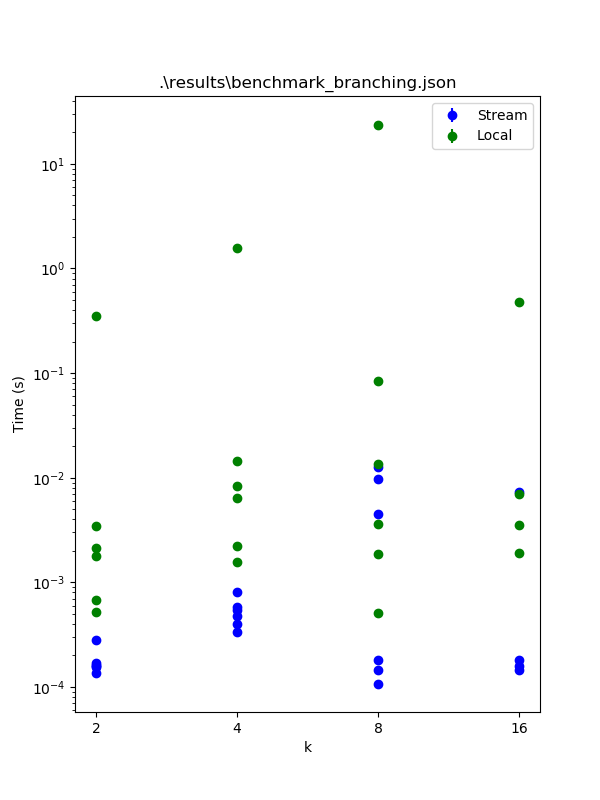
\includegraphics[width=\textwidth]{benchmark_time_branching.png}
    \caption{Runtimes of Branching}
    \label{fig:benchmark_time_branching}
\end{figure}

Figure \ref{fig:benchmark_time_branching} shows the runtimes of the branching
methods. Due to the branching algorithm having a runtime of \(O(2^k)\), it
quickly became clear that we were not going to be able to gather as much data as
we had initially wanted. Fortunately, the data we were able to gather paints
much the same picture as the kernelization algorithms.

\subsection{Stream Implementation}

We built a graph streaming platform on top of Faust and Apache Kafka. Faust is
a Python stream processing library for use with Kafka. The platform consists of
one Faust instance serving as both the processor performing the algorithms and
as a web server, and a second Faust instance serving as the source of the graph
stream. The web server serves a front end, shown in Figure
\ref{fig:stream_font_end} to clients. From here, users can create processing
jobs by selecting the algorithm, graph, and a \(k\) value from the top left
box. On submission of a job, the middle column shows the streamed edges down
the middle column and, on completion, the right column displays a log of
results of each job. In early iterations of the system, logging every edge from
the incoming stream would freeze the entire site until the stream was finished.
Due to this, the stream log has been throttled in the number of updates it is
allowed to display per second and so should not be used as a true log as some
edges from the stream will be skipped. It has been left there as a visual cue
that an algorithm is running, plus it is interesting to see the data being
processed.

\begin{figure}[htb]
    \centering
    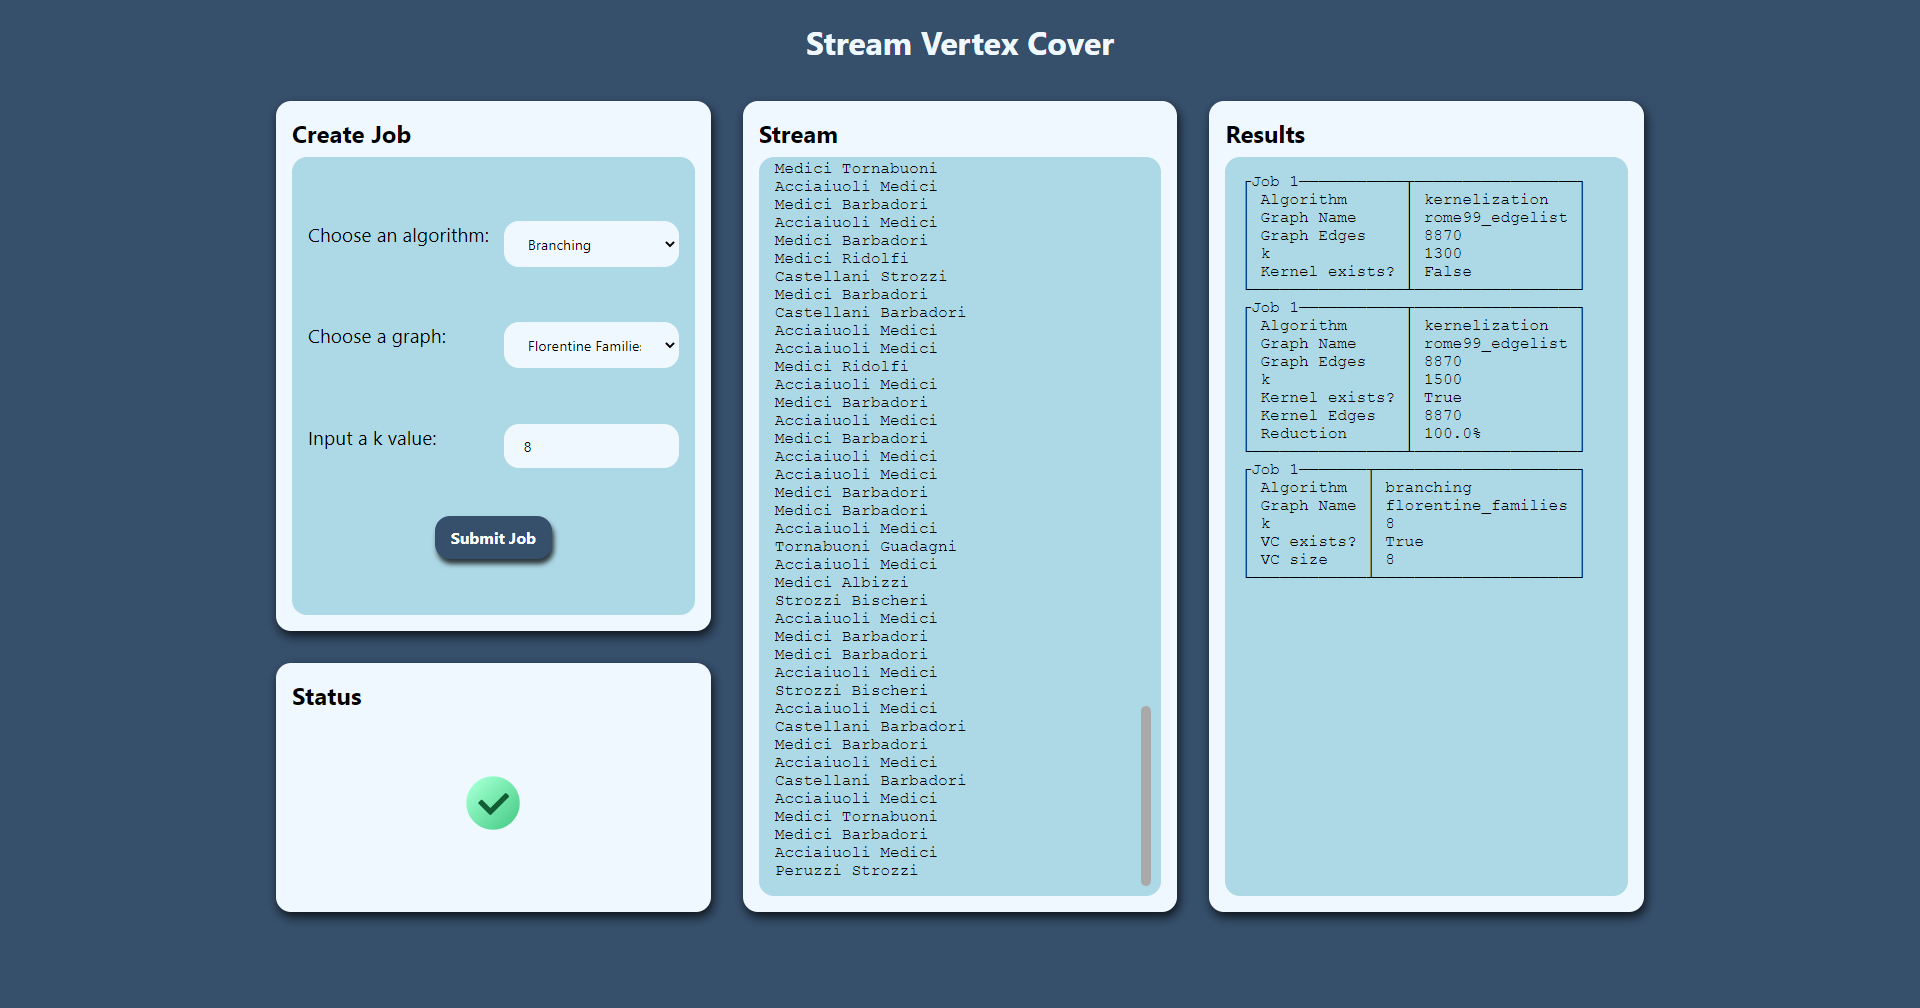
\includegraphics[width=\textwidth]{stream_new.png}
    \caption{Stream Implementation Front End}
    \label{fig:stream_font_end}
\end{figure}

The front end is built with HTML/CSS/JS and uses Server-Sent Events (SSE) for
the transmission of the stream and result logs. Originally, we had considered
using WebSockets, as the communication is bi-directional between the client and
server, but this introduced complexity in sorting through the different message
types (job submission/stream log/results log). It was deemed SSE was the better
option for the two logs, and then a HTTP POST request could be used for the job
submission.

As this is a proof-of-concept, the second Faust instance was built purely for
development purposes. Once a graph is requested, it streams the edge list from
a file and then relays that into a Kafka topic. In the development environment,
it is run locally, but because it's built with Kafka, it can be set up over a
network for a more typical production environment.

\subsubsection{Control Flow}

We have three actors present in our system:

\begin{itemize}
    \item
          App (Client) - The user's browser client
    \item
          App (Server) - The web server serving pages to the user and
          processing the algorithms
    \item
          Producer - The ``external'' server which is the source of the stream
          of graph edges
\end{itemize}

For the kernelization algorithm, the control flow is shown in Figure
\ref{fig:stream_kernelization}. The protocol used to communicate between each
actor is shown as a note covering between them.

\begin{figure}[htb]
    \centering
    \begin{minipage}{.5\textwidth}
        \centering
        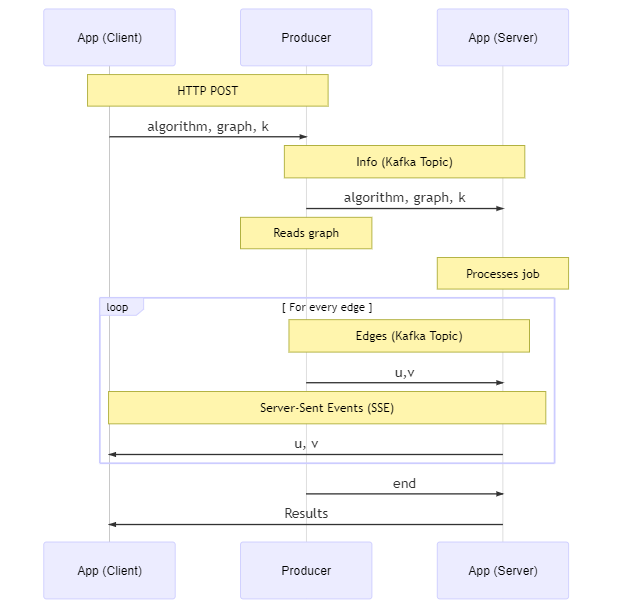
\includegraphics[width=\linewidth]{stream_kernelization.png}
        \captionof{figure}{Stream Kernelization Control Flow}
        \label{fig:stream_kernelization}
    \end{minipage}%
    \begin{minipage}{.5\textwidth}
        \centering
        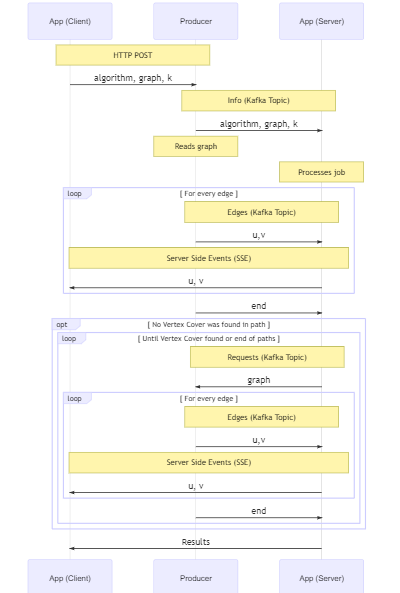
\includegraphics[width=\linewidth]{stream_branching.png}
        \captionof{figure}{Stream Branching Control Flow}
        \label{fig:stream_branching}
    \end{minipage}
\end{figure}

The branching algorithm requires a slightly different sequence of events
because it is a multi-pass algorithm. The sequence is shown in Figure
\ref{fig:stream_branching}. Some extra coordination is required for the server
to request the graph to be streamed again by the Producer.
